
\section{Introduction}
\label{sec:intro}

The increasing sophistication of generative models \cite{rombach2022high, AdobeFirefly, wu2025qwenimage} necessitates the development of reliable AI-generated image (AIGI) detectors to mitigate risks such as misinformation. An ideal detector must generalize to generated images from a wide array of generators. To this end, a common strategy is to expand the training dataset by aggregating data from multiple sources \cite{yang2025d3, park2025commfor} to turn the common \textit{Train on one} to \textit{Train on many}.

However, in the process of directly scaling up existing AIGI detector \cite{ojha2023towards,yang2025d3}, performance does not always increase as we wish. Instead, we observe a paradoxical phenomenon of \textit{\textbf{Benefit then Conflict}} in scaling up experiments; as illustrated in Fig.~\ref{fig:teaser} while aggregating data from a few generators is beneficial, the detector's efficacy diminishes as the diversity of training sources expands.  This counterintuitive outcome reveals fundamental limitations in scaling current AIGI detectors. To understand the underlying reason for this phenomenon, we construct a series of datasets equal number of generated images, but varying numbers of generators. Then we use a Linear Discriminant Analysis (LDA) model to assess the intrinsic separability in existing detectors, revealing two conclusions: (1) scaling itself causes data towards inseparable, (2) training in an end to end manner, which thought usually to be overfitting in domain, outperforms pretrained-based ones in scaling up setting. Based on these findings, we identify two primary challenges: \textit{\textbf{(1) Data-Level Heterogeneity}}: The feature distributions of images from different generators are highly diverse thereby amplifying the intrinsic difficulty of the classification task. As shown in Fig.~\ref{fig:teaser}(a), this inseparability cause a irregular decision boundary in detectors.  \textit{\textbf{(2) Model-Level Bottleneck}}: Many state-of-the-art detectors \cite{ojha2023towards, liu2024forgery, tan2025c2p, yan2024sanity, wen2025spot} rely on fixed, pre-trained encoders (e.g., CLIP \cite{CLIP})  for feature extraction. While these models provide powerful semantic priors to achieve generalization when training on single source, these priors may be contradictory when learning from heterogeneous data. As shown in Fig.~\ref{fig:tsne}, with only one generator, the fixed CLIP embedding space shows a clear decision boundary. However, when the number of generators increases to thousands, the features exhibit significant embedding overlap.

% To address these challenges, we pivot from the paradigm of unconstrained data aggregation to a more structured philosophy: \textit{Turn Thousands into a Few}. We realize this through our proposed \textbf{Generator-Aware Prototype Learning (GAPL)} framework. Instead of treating all forgery sources equally, GAPL is designed to learn a compact and robust representation of forgery itself. First, to counter \textit{data-level heterogeneity}, it learns a small set of prototypes from a few canonical generators. Each prototype represents a distinct, canonical forgery pattern. \textbf{Prototype Mapping (PM)} mechanism integrates prototypes and image embedding by reconstructing the embedding as a linear combination of prototypes weighted by the similarity. This design constrains the feature variance within the range defined by the prototypes, alleviating the heterogeneity of large scale data. Second, to break the \textit{model-level bottleneck}, GAPL adopts a two-stage training scheme that progressively integrates forgery cues into the model while preserving generalization brought by the pretrained encoder as much as possible. In the first stage we only train an MLP to transform the feature space forgery related, in the second stage we use LoRA \cite{hu2022lora} to tune a low-rank subspace that works synergistically with the PM mechanism. By overcoming the two key challenges, our model establishes a clearer and more generalizable decision boundary. In our comprehensive evaluation across 6 widely used benchmarks encompassing most popular generative models, our detector achieved an average performance of 90.4\% and an average accuracy of 94.9\%. This outperforms previous SoTA detector by 3.5\%. Moreover, in-depth experiments demonstrate the excellent robustness of our detector against post processing, thoroughly highlighting its applicability in real world.
To address these challenges, we propose \textbf{Generator-Aware Prototype Learning (GAPL)}, following a structured \textit{Turn Thousands into a Few} philosophy. Rather than treating all forgery sources equally, GAPL learns a compact representation of forgery. To handle \textit{data-level heterogeneity}, it learns a small set of prototypes from a few canonical generators, where each prototype captures a canonical forgery pattern. The \textbf{Prototype Mapping (PM)} mechanism reconstructs image embeddings as a linear combination of prototypes weighted by similarity, constraining feature variation within the prototype-defined space. To address the \textit{model-level bottleneck}, GAPL adopts a two-stage training scheme that injects forgery cues while preserving the pretrained encoder’s generalization. In Stage 1, an MLP is trained to make the feature space forgery-aware; in Stage 2, LoRA \cite{hu2022lora} tunes a low-rank subspace that works synergistically with the PM mechanism. Across six benchmarks, GAPL achieves 90.4\% average accuracy and 94.9\% average precision, outperforming the previous state of the art by 3.5\%. Moreover, in-depth experiments demonstrate the excellent robustness of our detector against post processing, thoroughly highlighting its applicability in real world.

Our contributions are summarized as follows:
\begin{itemize}
\item We identify and analyze the ``Benefit then Conflict'' paradox in scaling up setting, revealing the core challenges that impede the scalability of current AIGI detectors.
\item We introduce Generator-Aware Prototype Learning (GAPL), a novel framework that effectively manages the high heterogeneity of AI-Generated images by learning a shared space of forgery prototypes.
\item Our method overcomes the limitations of fixed feature extractors by explicitly training a model to map diverse artifacts to a set of canonical forgery concepts, enabling a more robust and well-defined decision boundary.
\item Through extensive experiments, we demonstrate that GAPL achieves state-of-the-art performance, showing a consistent detection across benchmark with a mean accuracy of 90.4\% across 55 test subsets in 6 benchmarks, outperforms existing detectors.
\end{itemize}

\begin{figure}
    \centering
    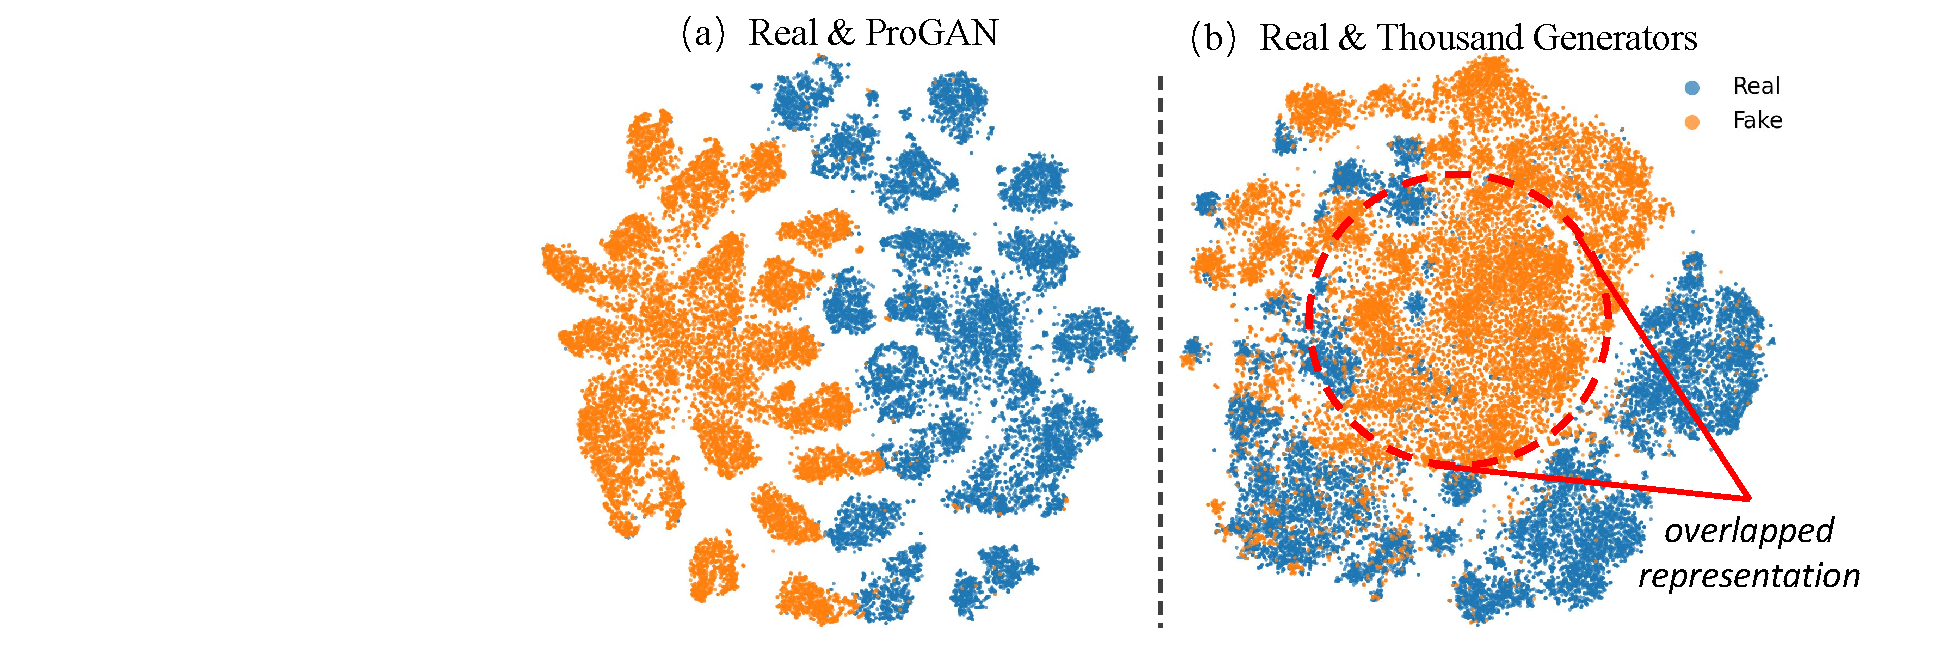
\includegraphics[width=1.0\linewidth]{figs/tsne.pdf}
    \caption{\textbf{T-SNE visualization on CLIP Embeddings.} \textbf{(a)} Comparison between images generated by a single generator and real images. \textbf{(b)} Comparison between images generated by thousands of diverse generators and real images.}
    \label{fig:tsne}
\end{figure}

